\subsection{Premises}\label{subsec:premises}

In this review,
I aim to provide a comprehensive overview of the research current state on security in autonomous vehicles,
in particular autonomous cars.
My focus is on the key cybersecurity threats, standards, and industry practices in the field,
keeping in mind that the landscape is rapidly evolving.
The goal is to identify the most critical challenges and opportunities for future research in this area
and underline the importance of a multi-layered approach to cybersecurity in AVs, starting from the design phase.
The ethical implications of the technology or the comparison between human-driven and autonomous vehicles in terms of accidents and fatalities will not be covered,
also social implications will not be deepened.

\subsection{Research Question}\label{subsec:research-question}

Starting from an introduction to the main threats in terms of cybersecurity regarding AV, the review will analyze the main actual opportunities to improve and regulate the security of these systems.
After that, the review will focus on the industry standards concluding in the future trends and emerging technologies that could enhance and simplify the security process of AVs.
This review address the following research questions:

\begin{enumerate}
    \item \textit{What are the most significant cybersecurity threats facing autonomous vehicles, and how these threats evolve with advancements in VANETs communications or with the evolution of the perception system of these vehicles?}
    \item \textit{What existing standards and regulatory frameworks address cybersecurity by design in autonomous vehicles, and are they enough to effectively tackle current and future security challenges?}
    \item \textit{What solutions and practices have been implemented by autonomous vehicle manufacturers, and how do they align with best practices in secure software development and system resilience?}
    \item \textit{What future trends and emerging technologies, such as artificial intelligence and blockchain, are being explored to enhance the cybersecurity of autonomous vehicles?}
\end{enumerate}

\subsection{Selection Criteria}\label{subsec:selection-criteria}

The selection criteria for the literature review are as follows:
\begin{enumerate}
    \item \textit{Relevance:} The literature must be directly related to the topic of security in autonomous vehicles, focusing on cybersecurity threats, standards, and industry practices.
    \item \textit{Quality:} The literature should be published in reputable journals, conference proceedings, or books, ensuring high academic and technical standards.
    \item \textit{Recency:} The literature should be recent (published within the last five years) to reflect the latest developments in the field.
    Some references can be not recent enough to be included in the last five-year filter, but they are fundamental to understanding the historical context or some specific technology.
    \item \textit{Diversity:} The literature should cover a broad range of topics within the field of autonomous vehicle security, including but not limited to threat modeling, risk assessment, secure software development, and hardware security.
    At the same time, the literature should be representative and inherently connected to the cybersecurity topic.
    \item \textit{Accessibility:} The literature should be accessible online or through academic libraries to ensure that it can be reviewed and cited effectively.
\end{enumerate}

\subsection{Search Strategy}\label{subsec:search-strategy}

The search strategy for this review involved a systematic exploration of electronic databases, books, and relevant publications.
The following databases were used to identify relevant literature:

\begin{enumerate}
    \item Google Scholar
    \item IEEE Xplore
    \item WebOfScience
    \item SpringerLink
\end{enumerate}

Multiple searches were conducted, initially to discover in general the state of the art in the field of autonomous vehicles and then to focus on the security aspects.
The search terms used included combinations of the following keywords:
\textit{autonomous vehicles},
\textit{self-driving cars},
\textit{cybersecurity},
\textit{security threats},
\textit{standards},
\textit{industry practices},
\textit{V2X communication},
\textit{ISO/SAE 21434},
\textit{UNECE WP.29 R155},
\textit{secure software development},
\textit{intrusion detection},
\textit{over-the-air updates},
\textit{artificial intelligence},
\textit{digital twins},
\textit{blockchain}.

Some principal queries were:
\begin{enumerate}
    \item \textit{autonomous vehicles cybersecurity threats}
    \item \textit{autonomous vehicles cybersecurity by design}
    \item \textit{autonomous vehicles cybersecurity standards}
    \item \textit{autonomous vehicles cybersecurity connectivity}
    \item \textit{autonomous vehicles cybersecurity perception sensors}
    \item \textit{autonomous vehicles cybersecurity architecture}
    \item \textit{autonomous vehicles cybersecurity accidents}
    \item \textit{autonomous vehicles cybersecurity V2V, V2I, V2X}
    \item \textit{autonomous vehicles cybersecurity future trends}
    \item \textit{secure software development lifecycle autonomous vehicle}
    \item \textit{autonomous vehicles secure over-the-air}
    \item \textit{autonomous vehicles cybersecurity future directions}
    \item \textit{autonomous vehicles cybersecurity privacy blockchain}
    \item \textit{autonomous vehicles cybersecurity artificial intelligence}
\end{enumerate}

Moreover, some filter was applied to search only recent results, only peer-reviewed articles, and only articles in English.
First, the search was conducted on Google Scholar and IEEE Xplore, used like entry points to the other databases.
In other cases, instead, a direct search on institutional websites was conducted to find specific standards or reports (e.g. \url{https://www.sae.org/}, \url{https://unece.org/wp29-introduction}).

The search strategy aimed to identify a diverse range of sources, including academic papers, conference proceedings, books, and industry reports, to provide a comprehensive overview of research on security in autonomous vehicles.
In certain cases, as already mentioned, the limit on the age of the publication was removed to include fundamental works that are not recent but representative of a specific technology or approach (e.g. CAN bus).
Moreover, some references are relative to the automotive industry in general, but they are fundamental to understanding the context in which autonomous vehicles are developed.

\subsubsection{Phases}\label{subsubsec:phases}
The search of papers and documents was conducted in two phases:
\begin{enumerate}
    \item \textit{General Search:} The initial search aimed to identify the main topics and subtopics related to cybersecurity in autonomous vehicles, helping to understand the current state, main threats and some general aspects of the AVs.
    \item \textit{Specific Search:} The second search focused on specific aspects of cybersecurity in autonomous vehicles, such as specific threats, standards, industry practices, techniques, and then future trends.
\end{enumerate}

Every search was conducted using the same base keywords and filters.
To ensure consistency and comparability of results across different databases, in particular, the keywords \textit{autonomous vehicles} and \textit{cybersecurity} were always present in the search query to keep the focus on the main topic of the review.
Only for the~\ref{sec:future-directions} section, a two-year filter was applied to ensure the most recent results but not excluding other works.

In case of doubt about the relevance of a paper, the paper was read to understand if it was pertinent to the topic of the review.
The number of citations was also considered but not like a primary filter, favoring instead the quality of the paper and the relevance in terms of cybersecurity of the content.
Another important aspect is that social, ethical, and legal implications were not considered, so the papers focused on these aspects were excluded.


\subsection{Quality Assessment}\label{subsec:quality-assessment}
The quality assessment of the selected literature has been differentiated based on the type of citation.
For books, the evaluation has been based on the reputation of the author and the publisher, considering both their academic credentials and contributions to the field.
Additionally, like for the entire literature, the relevance of the book to the specific topics of cybersecurity and autonomous vehicles has been taken into account.

Given the interdisciplinary nature of this topic, many social sciences and related fields works are present but not considered if not for the brief historical and social implications' context.
The grade of confidence for principal papers has been evaluated based on several factors:
the demonstration of results, coherence of conclusions, and the methodology employed.

Articles that provide empirical data or case studies have been weighted more heavily, as they offer concrete evidence to support theoretical claims.
The citation index and impact factor of journals have also been considered but not prioritized over the relevance and quality of the content.

This approach ensures a comprehensive understanding of the topic, acknowledging the complexity of cybersecurity challenges without losing the focus.

\subsection{Data Extraction}\label{subsec:data-extraction}

The data extraction process involved identifying key information from the selected literature to address the research questions.
The following data points were extracted from each source:
\begin{enumerate}
    \item \textit{Publication:} The title of the publication, including the journal, conference, or book where the work appeared.
    \item \textit{Year:} The publication year to determine the recency of the source.
    \item \textit{Research Focus:} A brief summary of the main research focus or objective of the publication.
    \item \textit{Key Findings:} The primary findings or results of the research, including any significant insights or conclusions.
    \item \textit{Methodology:} The research methodology employed in the study, such as case studies, surveys, experiments, theoretical analysis and proposals.
    \item \textit{Relevance:} The relevance of the publication to the research questions and the broader topic of cybersecurity in autonomous vehicles.
\end{enumerate}

\subsection{Limitations}\label{subsec:limitations}

The limitations of this review include the following:
\begin{enumerate}
    \item \textit{Scope:} The review focuses primarily on cybersecurity threats, standards, and industry practices in autonomous vehicles, excluding ethical, legal, and social implications.
    Moreover, the review focuses on the main threats, not considering all the possible attacks due to the complexity and always evolving nature of the field.
    \item \textit{Recency:} Due to the rapidly evolving nature of the field, some literature may not capture the most recent or current techniques in autonomous vehicle security (e.g. machine learning algorithms) but address the main common solutions.
    \item \textit{Accessibility:} The availability of certain publications may be limited, but access to academic databases and libraries minimized the issue.
    \item \textit{Interdisciplinary nature:} The interdisciplinary nature of the topic may present challenges in synthesizing findings from diverse fields, but efforts have been made to ensure a comprehensive and holistic review.
\end{enumerate}

\subsection{Motivation}\label{subsec:motivation}

Some historic major attacks highlighted the importance of security in AV systems.
As a result, both manufacturers and researchers recognized the need to strengthen security measures.
This realization led to an emphasis on improving security by design.
Some proposal to hardening security in AVs will be analyzed; moreover, standards that are trying to regulate the security of these systems from the design to the deployment will be compared.
The problem and the motivation are that the security of AVs is a complex issue to be solved by a single solution and without the collaboration of all the stakeholders\cite{comparison-standard}.
The goal is to provide a holistic vision of the main threats and the current solutions on which the researchers are focusing on the cybersecurity field
analyzing main sensors composing the perception system and the VANETs communication system.

\newpage
\subsection{Structure of the Survey}\label{subsec:structure-of-the-survey}
\begin{figure}[!htb]
    \centering
    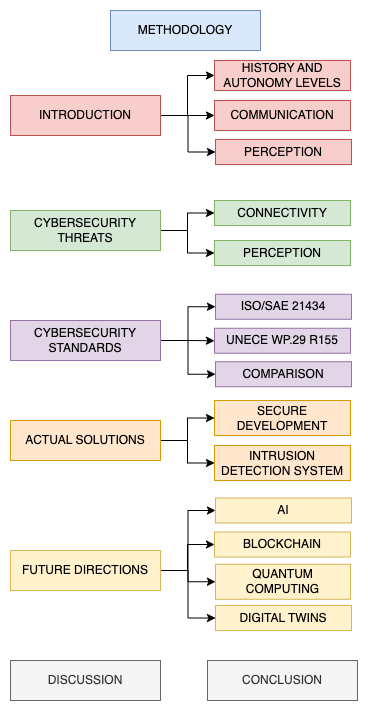
\includegraphics[width=0.6\linewidth]{figures/survey-structure}
    \caption{Survey structure}
    \label{fig:survey-structure}
\end{figure}
\newpage
